\documentclass[10pt, conference, compsocconf]{IEEEtran}


\makeatletter
\newcommand\figcaption{\def\@captype{figure}\caption}
\newcommand\tabcaption{\def\@captype{table}\caption}
\makeatother


\ifCLASSINFOpdf
 \usepackage[pdftex]{graphicx}
 
\else
 
\fi
\hyphenation{op-tical net-works semi-conduc-tor}


\begin{document}

\title{A light-weight secure protocol for small data dissemination in WSN}

\author{\IEEEauthorblockN{Wang Yan}
\IEEEauthorblockA{School of Computer Science and Software Engineering \\
East China Normal University\\
Shanghai, China\\
boliangzai@foxmail.com}
\and
\IEEEauthorblockN{He Daojing}
\IEEEauthorblockA{School of Computer Science and Software Engineering\\
East China Normal University
\\
Shanghai, China\\
djhe@sei.ecnu.edu.cn
}
}

\maketitle


\begin{abstract}
This paper argues for a super lightweight, confidential and Dos-resistant broadcast authentication mechanism and its high efficiency in securing Drip protocol, an open source small data dissemination protocol in Wireless sensor Network. 

In Wireless Sensor Networks, WSNs, dissemination is typically used to query nodes, send commands, and reconfigure the network. It's important to protect WSNs from vicious data sent by attackers. But in terms of bandwidth, storage and computing consumption, it's  expensive to implement authentication and confidentiality using typical cryptographic mechanisms like ECDSA, RSA.  Based on these observation, this paper presents security requirements for broadcast authentication in WSNs. Efficiency problem and security weaknesses of existing broadcast authentication methods are also included in our research.

We believe our work is able to make whole network immune to Dos attack and Sybil attack. 

\end{abstract}

\begin{IEEEkeywords}
component; formatting; style; styling;

\end{IEEEkeywords}


\IEEEpeerreviewmaketitle



\section{Introduction}
% no \IEEEPARstart
WSN consists of a lot of space distributed sensors. And to obtain valuable information about physical world, WSN needs broadcast message to every node in the network. As a result, message secrecy becomes very important while communication channels are shared among all users. Besides, the issue that life and safety are involved in some of these applications makes authentication of broadcast messages much more important. As shown in Fig.1.  Attacers are able to intercept messages and send vicious message to receiver nodes.

\begin{figure}
\centering
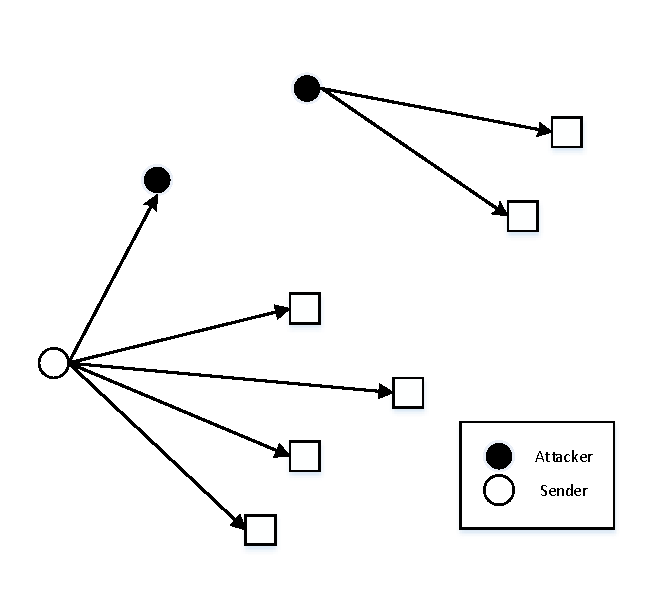
\includegraphics[width=4cm,height=4cm]{fig_1.pdf}\\
\caption{Fig.1}\label{} 
\end{figure}
It has become critical to develop a mechanism including authentication and confidentiality.
On one hand,  broadcast authentication scheme must ensure that broadcast messages are received directly from dependable sources. On the other hand, receivers don't want receive   modified messages in transit.

In order to make broadcast message secure, our paper has three main contributions.

1) Analyses of requirements for a secure broadcast mechanism in smart grids and their security weaknesses as well as efficiency problems.

2) Development of a secure, lightweight, robust ,confidential and DoS-resistant broadcast authentication mechanism for smart grids. 

3) Implementation of the proposed protocol in networks of Telosb motes. Experimental results demonstrate high efficiency and performance.

The rest of the paper is organized in the following manner. In Section II, we review the various existing broadcast authentication protocols. Section III presents the network model, security requirements and assumptions, highlights the challenge of broadcast authentication. Section IV describes the proposed protocol in detail after definition of some preliminaries of cryptography. Section V analyses the security and efficiency properties of our protocol. Section VI describes the implementation and experimental results of the proposed protocol via real sensor platforms. Finally, Section VII concludes this paper.


\section{Related work}
Data dissemination is within the scope of broadcast authentication.
There is a lot of challenges on providing security in our smart grid. The primary one is the limited computing, communication and storage capabilities of receivers. A message authentication code (MAC) is usually an authentication tag derived by applying an authentication scheme and a secret key to a  message.
MAC is an efficient symmetric cryptographic primitive for two-party authentication, but it is not suitable for broadcast communication. Because the sender and its receivers share the same secret key, any one of the receivers can impersonate the sender and forge vicious messages to other receivers. Which means asymmetric mechanisms is more suitable for broadcast authentication. More exactly, the sender signs each packet individually using digital signature technique and each receiver verifies the signature before processing the packet. The signature is vulnerable to Dos attacks. That is, the adversary may flood a large number of illegal packets to receivers to exhaust their limited resources and render them less capable of serving legitimate users. To provide authentication, some researchers proposed TESLA and its various extensions to authenticate broadcast packets in a network [7][9]. It employs symmetric cryptography primitives with delayed key disclosure to achieve the effect of asymmetric mechanism, more specifically, the key used to authenticate current message is to be disclosed in next  message. However these methods requires time synchronization in the whole network, which leads to more complicated measures to secure synchronization. In addition, the receivers cannot authenticate packets immediately, but have to wait until the respective keys are disclosed, resulting in excessive verification latency and a requirement to store unauthenticated packets. What's more, this protocol has some disadvantage, such as, non-repudiation, one-way key chain that has a predefined-length, short duration.   Dos attack
\cite{a} and non-repudiation. Some other researchers proposed one-time signature schemes. Unfortunately, such schemes suffer from large key size and a limited number of keys is available.{Biba}

Recently, since packet contains signature  means a big consumption in delivery, some signature amortization protocol, EMSS, has been proposed.. With EMSS\cite{efficient}, periodic signature pakcets are sent after every N data packets. Thus, all the packets that arrive before their signature packet have to wait to be verified.
In another protocol \cite{aspect} , First packet contains a signature of next packet, signature is signed on hash of next packet, and recusively, current packet contains hash of next packets. 


\section{Problem definition}
\subsection{Network Model}
We consider a broadcast group involving one sender (S) and
a group of receivers (R i ). Each message is delivered from S to
each R through lossy and insecure PLC network, as illustrated
in Fig. 4. The intermediate receivers in the network only
forward the packets and do not provide any security measure
(such as integrity and authenticity checks). These receivers
may also be malicious and drop or modify S’s packets or
even inject fake packets.
We consider a class of applications where 1) each generated
message is unknown to S until it is ready to send; 2) S
(resp. R) signs (resp. verifies) the message once it appears;
3) the sending rate at S is dynamic. The data flow of the
broadcast authentication protocol is shown in Fig. 5.

\subsection{requirement}

In addition to the asymmetric mechanism that is needed
for broadcast authentication, an efficient and secure broadcast
authentication scheme for smart grids should still satisfy the
following requirements:

1) Individual authentication: The receiver should verify
the received packets individually without depending onother packets; otherwise, the failure to verify a packet
prevents the verification of subsequent packets.

2) Robust to packet loss: The smart grid communication
environment is not reliable; therefore, the scheme should
be able to cope with the loss of packets during trans-
mission.

3) Short authentication latency: Many PLC applications are
real time applications, e.g. sending the control informa-
tion to the customers. To authenticate real time data, the
maximum number of additional packets that need to be
received before a packet can be authenticated should be
small.

4) Low computation cost: Receivers have limited compu-
tation power. Thus, they should only perform a small
number of operations to verify a packet.

5) Receiver compromise tolerance: The protocol should be
resilient to receiver compromise attack no matter how
many receivers have been compromised, as long as the
subset of non-compromised receivers can still form a
connected graph with the trusted source.

6) Low communication overhead: Because a PLC network
often is restricted in bandwidth, the number of bytes per
packet used for authentication should be small.

7) DoS attacks resistance: The functions of the PLC net-
work should not be disrupted by DoS attacks.

8) Freshness: A receiver should be able to differentiate
whether an incoming message is the newest version.

9) Scalability: The protocol should be efficient even for
large-scale smart grids with thousands of receivers.

10) Low storage requirement: Since the storage space of
receivers is limited, some data for authentication like
key material and signatures stored in memory cannot be
too large.

11) Data Confidentiality: In some critical applications, the
data items from the sender are strictly private and
confidential. They should be encrypted to protect the
data privacy from eavesdroppers. If the broadcast data
items are chosen from a small finite set, the encryption
should produce ciphertext that does not give information
to an intruder on which of these messages was sent.
Ideally, we would like a scheme that recovers from any
loss of packets, has no authentication latency, can individually
authenticate packets and ensure data confidentiality, has neg-
ligible overhead, and has a low computation cost. In practice,
such a perfect scheme is difficult to achieve, and a compromise
needs to be found between these requirements.
\subsection{Assumptions}
Our protocol makes the following assumptions.

• The sender cannot be compromised, and is trusted. In
Drip, the sender is the origin of all legitimate message
updates. The sender has unlimited computational power
compared with receiver.

• The receiver can perform a limited number of asymmetric
cryptographic operations such as signature verification in
TinyECC [15], but they cannot afford to perform many
such operations due to their energy limitations.


\section{THE PROPOSED PROTOCOL}
Before explaining our protocol in detail, we provide an overview of our protocol in advance.
\subsection{Overview of Our Protocol}
Within public key cryptography systems, elliptic curve cryptography (ECC) has many merits such as small key size, high computational and communication efficiency. But On TinyOS platforms it still need a relatively long time to execute.  That means any protocol using ECC is vulnerable to DoS attack. Many protocols to alleviate this kind of situation have been proposed. Some researchers employed the message specific puzzle and included the puzzle in message packet\cite{Msp}. 

In our protocol we propose cipher puzzle to integrate confidentiality and DoS-resistance. The computational efforts of these two puzzles for the sender are the same. But the difficulty for an adversary to construct a valid puzzle solution is different. In MSP, the demand of a specific puzzle is a fixed segment, e.g. the first V bytes of the result is 0, such that a attacker can launch brute force to find a solution to puzzle and hence forge bogus message to control the whole network.

In CP, the first V bytes of the hashed result is equal to another hashed result. Because of the uncertainty, it's hard for attackers to brute force for an solution. In addition, all the messages to be authenticated are unencrypted. A adversary can readily intercept the communications in network to obtain these messages without compromising receiver node.

Considering confidentiality of key, if we set key on receiver node directly, attacker can compromise our nodes and get our key and hence forge a vicious message to control our network.

So we don't put all information about our key on receiver node, we only put some segment of key on receiver node. 

Our protocol consists of three phases: system initialization, packet pre-processing, and packet verification. The system initialization phase is carried out before network deployment. In this phase, the sender creates the key materials, and loads the public parameters on each receiver. Then before disseminating a data item, the sender executes the packet pre-processing phase in which a data packet is constructed. Finally, in the packet verification phase, a receiver verifies each received packet. If the result is positive, it updates the data according to the received packet. In the following, each phase is described in detail. The notation used in describing our protocol are listed in Table I.

\begin{table}[!htp]
\begin{tabular}{l l}

\hline
Notation & Description  \\
\hline
\emph{SIG}$_k$(\emph{M}) & the signature on message \emph{M} with key \emph{k} \\
\emph{E}$_k$(\emph{M}) & encryption message \emph{M} with a symmetric key \emph{k}\\

$,$ or $||$ & concatenation operator of the two bit streams\\

\emph{H}(.) & public one-way cryptographic hash function (e.g., SHA-1)\\

\emph{H}(\emph{M}) & the hash value of message M\\
\end{tabular}

\caption{NOTATIONS}
\end{table}
\subsection{System Initialization Phase}

In Drip, every data item has 3 tuple. (data, version , key) data is the data you want the whole WSN to update. version demonstrates the new or old of your data. key uniquely identifies the data item. So this 3 tuple is the message we need to protect and distinguish it from other vicious message. Others cannot forge our message.  Same as the Drip implementation, key and version are 2 bytes and 4 bytes long respectively. 

\begin{figure}
\centering
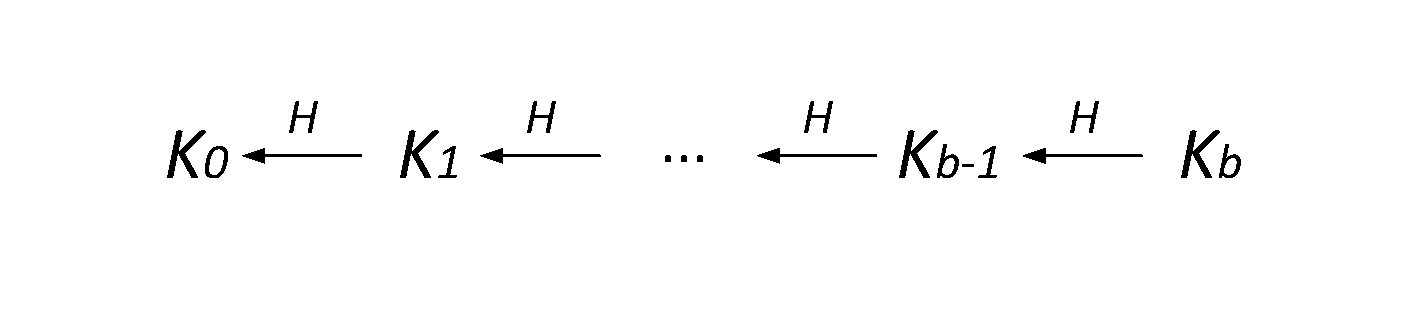
\includegraphics[width=8cm]{Hash_chain.pdf}\\
\caption{Fddddd}\label{11} 
\end{figure}



\section{Conclusion}
The conclusion goes here. this is more of the conclusion


\section*{Acknowledgment}


The authors would like to thank...
more thanks here
\cite{IEEEhowto:kopka}
\cite{jour}
\cite{book}
\begin{thebibliography}{12}

\bibitem{IEEEhowto:kopka}
H.~Kopka and P.~W. Daly, \emph{A Guide to \LaTeX}, 3rd~ed.\hskip 1em plus
  0.5em minus 0.4em\relax Harlow, England: Addison-Wesley, 1999.


\bibitem{jour} Smith, T.F., Waterman, M.S.: Identification of Common Molecular
Subsequences. J. Mol. Biol. 147, 195--197 (1981)

\bibitem{a} Grover K, Lim A.: A survey of broadcast authentication schemes for wireless networks[J]. Ad Hoc Networks, 2015, 24: 288-316.

\bibitem{Biba} Perrig A.: The BiBa one-time signature and broadcast authentication protocol[C]//Proceedings of the 8th ACM conference on Computer and Communications Security. ACM, 2001: 28-37.

\bibitem{apsect} He D, Chan S C, Guizani M.: Small data dissemination for wireless sensor networks: The security aspect[J]. Wireless Communications, IEEE, 2014, 21(3): 110-116.

\bibitem{efficient} Perrig A, Canetti R, Tygar J D, et al.: Efficient authentication and signing of multicast streams over lossy channels[C]//Security and Privacy, 2000. IEEE Symposium on. IEEE, 2000: 56-73.%Here I delete S&P 2000

\bibitem{trickle}Patel N, Culler D, Shenker S.: Trickle: A self regulating algorithm for code propagation and maintenance in wireless sensor networks[M]. Computer Science Division, University of California, 2003.

\bibitem{lnicstchap} May, P., Ehrlich, H.C., Steinke, T.: ZIB Structure Prediction Pipeline:
Composing a Complex Biological Workflow through Web Services. In: Nagel,
W.E., Walter, W.V., Lehner, W. (eds.) Euro-Par 2006. LNCS, vol. 4128,
pp. 1148--1158. Springer, Heidelberg (2006)

\bibitem{book} Foster, I., Kesselman, C.: The Grid: Blueprint for a New Computing
Infrastructure. Morgan Kaufmann, San Francisco (1999)

\bibitem{proceeding1} Czajkowski, K., Fitzgerald, S., Foster, I., Kesselman, C.: Grid
Information Services for Distributed Resource Sharing. In: 10th IEEE
International Symposium on High Performance Distributed Computing, pp.
181--184. IEEE Press, New York (2001)

\bibitem{proceeding2} Foster, I., Kesselman, C., Nick, J., Tuecke, S.: The Physiology of the
Grid: an Open Grid Services Architecture for Distributed Systems
Integration. Technical report, Global Grid Forum (2002)

\bibitem{url} National Center for Biotechnology Information, http://www.ncbi.nlm.nih.gov

\bibitem{Msp}He D, Chan S C, Tang S, et al. Secure Data Discovery and Dissemination based on Hash Tree for Wireless Sensor Networks[J]. IEEE Transactions on Wireless Communications, 2013, 12(9):4638-4646.
\end{thebibliography}


\end{document}


